\documentclass{article}
\usepackage{graphicx}
\usepackage[shortlabels]{enumitem}
\usepackage{subcaption}
\usepackage{amsmath}

\begin{document}

\section{Cylindrical Dam Break Collapse using Newton-Raphson Variable-h SPH}
\subsection{Comparison with Vishnu's Simulation}
\begin{itemize}
\item The Newton-Raphson Iterative procedure is implemented to find the
smoothing length of each particle such that its neighbors are approximately
constant.  
\item This is compared with Vishnu's simulation, wherein the smoothing length is
initially doubled and recalculated from the summation density and volume of the
particle.
\item For the dam break shown in Fig. \ref{fig:collapse}, the interior
particles have retained more of their circular arrangement on using the 
variable-h SPH with Newton-Raphson iteration.
\item For a final simulation time of 2s, the variable-h SPH using
Newton-Raphson iteration took 2.5 hrs whereas the other took 0.8 hrs.
\end{itemize}


\begin{figure}[!htbp]
\centering
\begin{subfigure}{.5\textwidth}
  \centering
  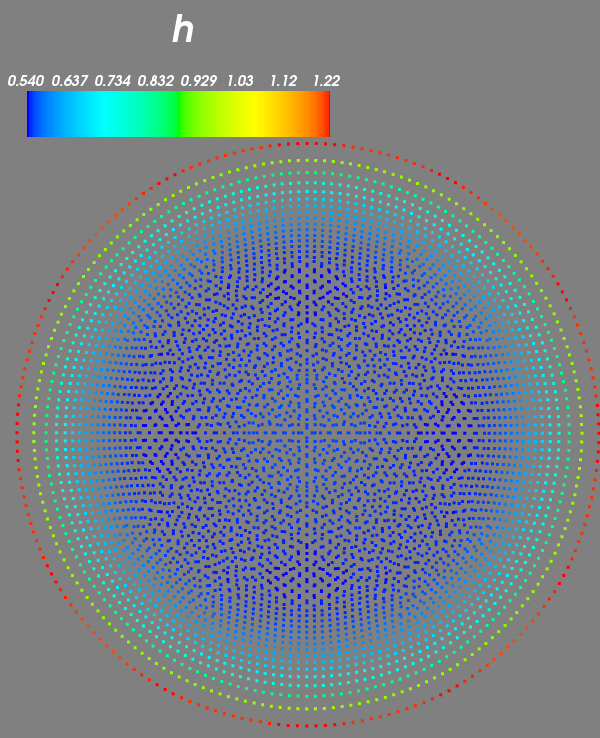
\includegraphics[width=0.85\linewidth]{vishnu_varh_circ_dam_break.png}
  \caption{Vishnu Simulation}
  \label{fig:sub11}
\end{subfigure}%
\begin{subfigure}{.5\textwidth}
  \centering
  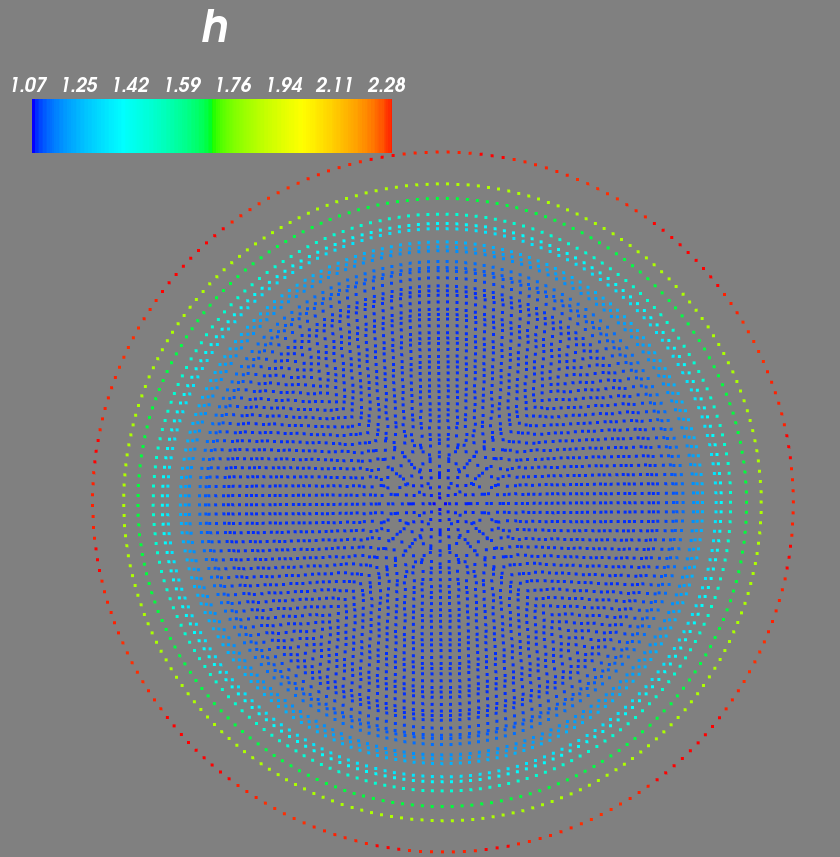
\includegraphics[width=1.0\linewidth]{My_varh_circ_dam_break.png}
  \caption{Variable-h SPH (Newton-Rapshon Iteration)}
  \label{fig:sub21}
\end{subfigure}
\caption{Top View of a Collapsing Water Column}
\label{fig:collapse}
\end{figure}
\newpage
\subsection{Comparison with Rodriguez dam break example}
\begin{itemize}
\item As shown in Fig. \ref{fig:sub13}, an initially cylindrical dam of
height 1m and dia 1m is made to collapse on a frictionless flat bed. Viscous
effects of the fluid have not been considered.
\item As shown in Fig. \ref{fig:sub1}, a perfectly flat cylindrical column height
could not be maintained as first the summation density was calculated and
then the height was computed based on below formula (Boundary particles having less density
and hence less height compared to interior particles due to kernel truncation effect)
\begin{equation}
h_t = \rho * 1000
\label{}
\end{equation}
\item Comparing the simulation results (Fig. \ref{fig:sidecollapse})  with the Rodriguez example (Fig. \ref{fig:sub13}) , it is observed that a good 
match is obtained for the fluid column height at various times.
\item Comparing the simulation results (Fig. \ref{fig:topcollapse})  with the Rodriguez example (Fig. \ref{fig:sub14}) , it is observed that a good 
match is obtained for the fluid column width at various times.
\end{itemize}
\begin{figure}[!htbp]
  \centering
  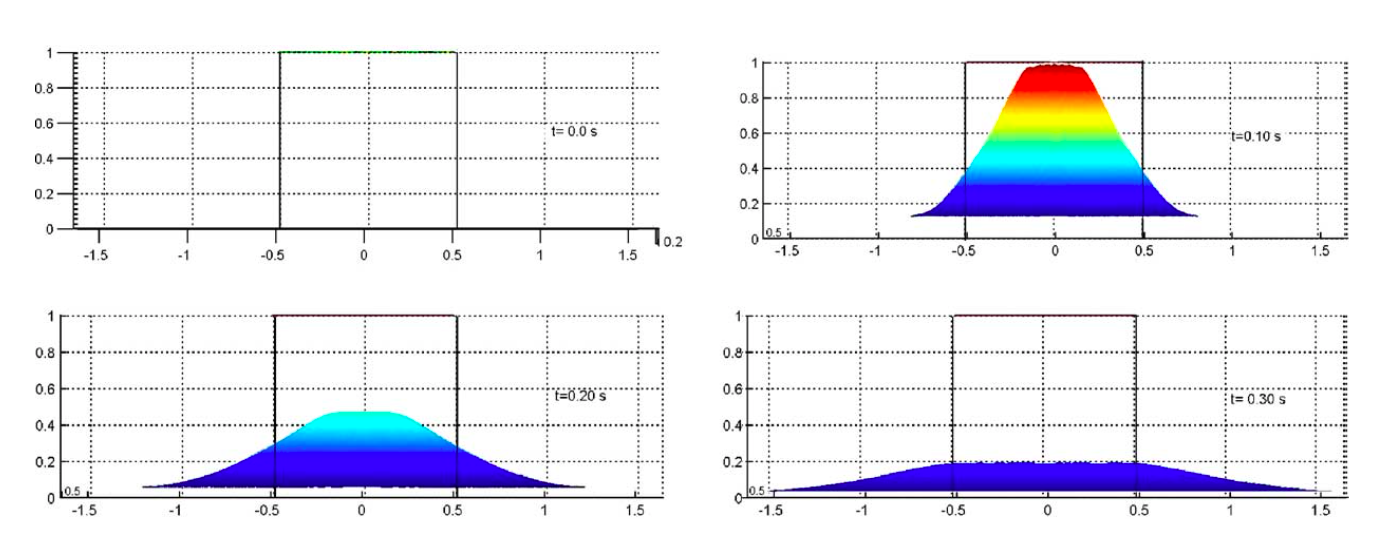
\includegraphics[width=1.1\linewidth]{rodri.png}
  \caption{Collapse of cylindrical water column (Reproduced from Rodriguez et al)}
  \label{fig:sub13}
\end{figure}


\begin{figure}[!htbp]
\centering
\begin{subfigure}{.5\textwidth}
  \centering
  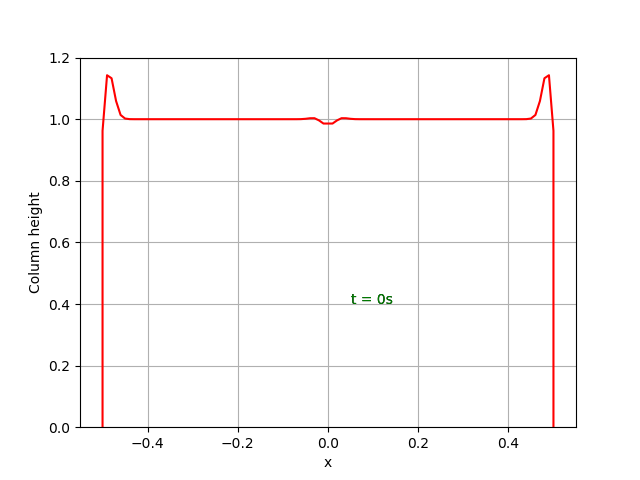
\includegraphics[width=1.1\linewidth]{circ_dam_t0.png}
  \caption{t = 0 s}
  \label{fig:sub1}
\end{subfigure}%
\begin{subfigure}{.5\textwidth}
  \centering
  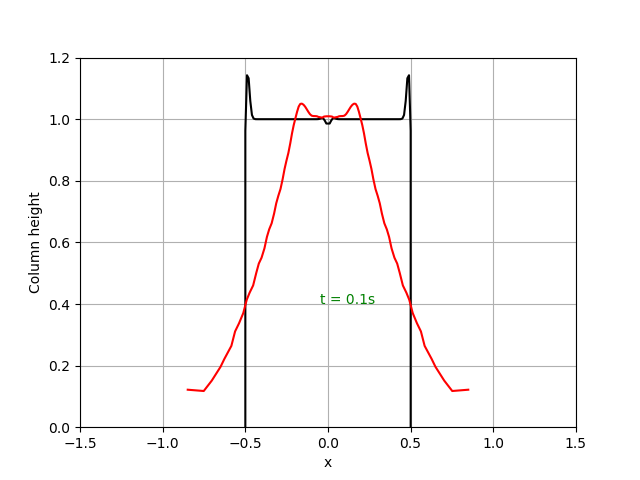
\includegraphics[width=1.1\linewidth]{circ_dam_t1.png}
  \caption{t = 0.1 s}
  \label{fig:sub2}
\end{subfigure}
\begin{subfigure}{.5\textwidth}
  \centering
  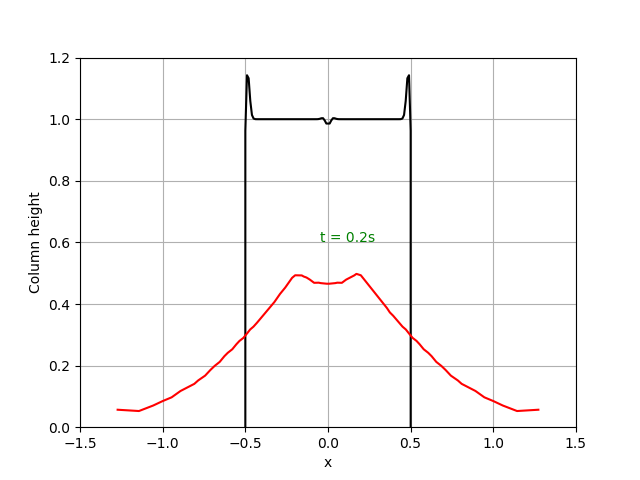
\includegraphics[width=1.1\linewidth]{circ_dam_t2.png}
  \caption{t = 0.2 s}
  \label{fig:sub3}
\end{subfigure}%
\begin{subfigure}{.5\textwidth}
  \centering
  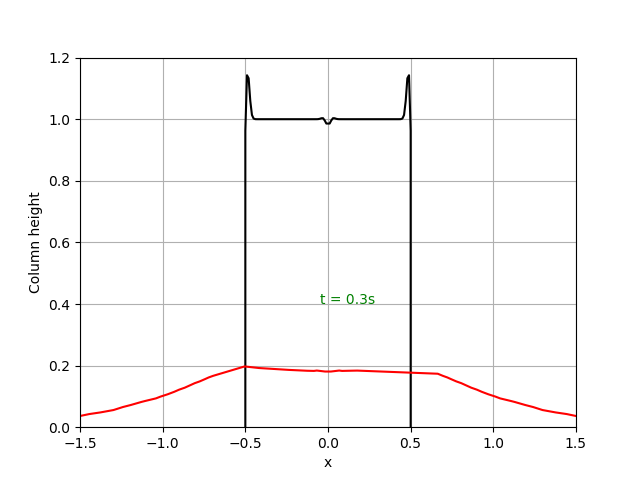
\includegraphics[width=1.1\linewidth]{circ_dam_t3.png}
  \caption{t = 0.3 s}
  \label{fig:sub4}
\end{subfigure}
\caption{Side View of a Collapsing Water Column}
\label{fig:sidecollapse}
\end{figure}

\begin{figure}[!htbp]
  \centering
  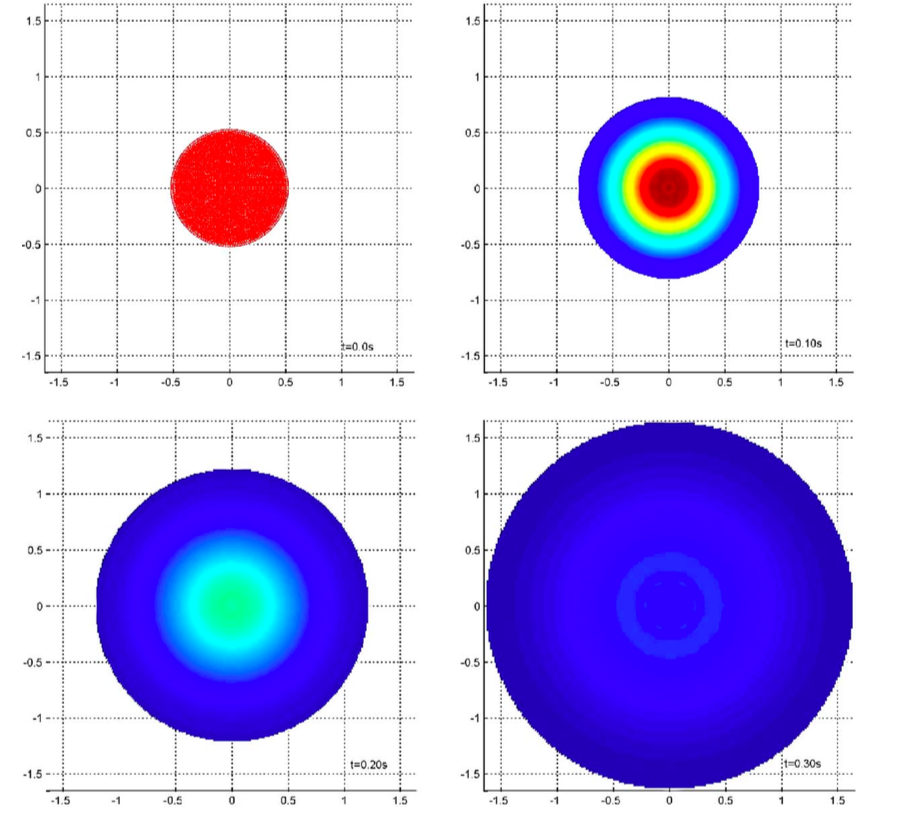
\includegraphics[width=1.1\linewidth]{rodri2.png}
  \caption{Top View of collapse of a cylindrical water column (Reproduced from Rodriguez et al)}
  \label{fig:sub14}
\end{figure}


\begin{figure}[!htbp]
\centering
\begin{subfigure}{.5\textwidth}
  \centering
  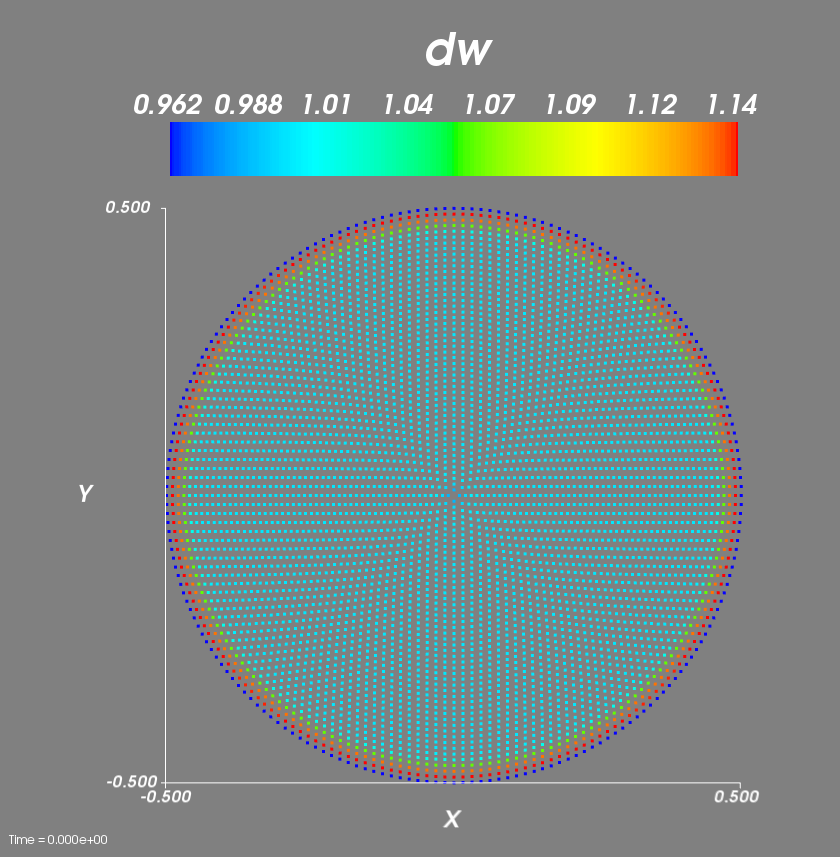
\includegraphics[width=1.1\linewidth]{width_t0.png}
  \caption{t = 0 s}
  \label{fig:su1}
\end{subfigure}%
\begin{subfigure}{.5\textwidth}
  \centering
  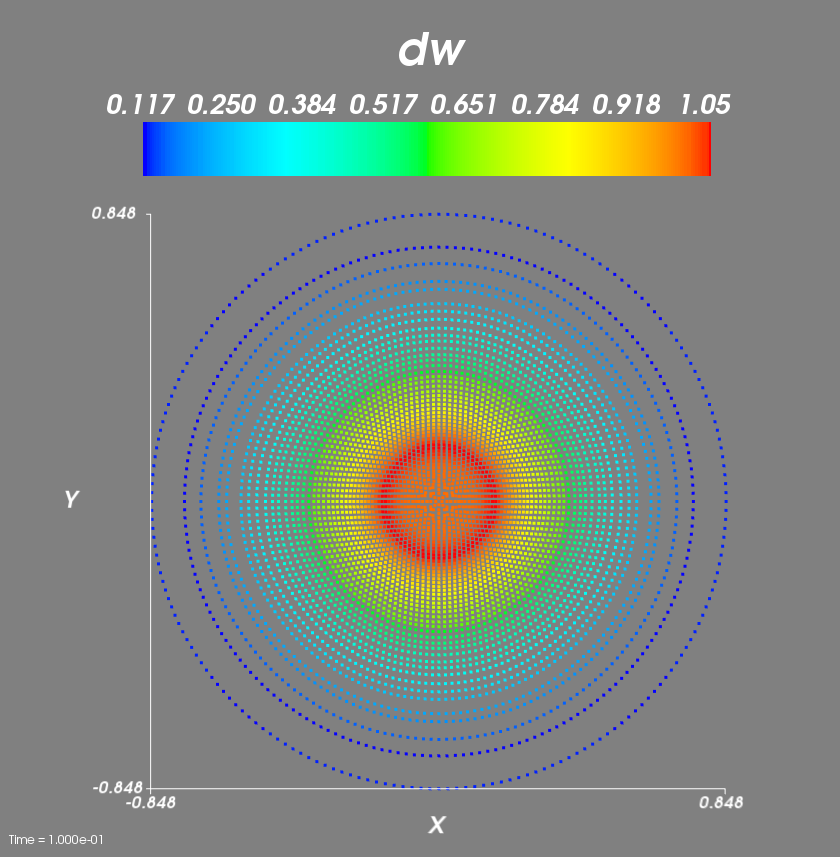
\includegraphics[width=1.1\linewidth]{width_t1.png}
  \caption{t = 0.1 s}
  \label{fig:su2}
\end{subfigure}
\begin{subfigure}{.5\textwidth}
  \centering
  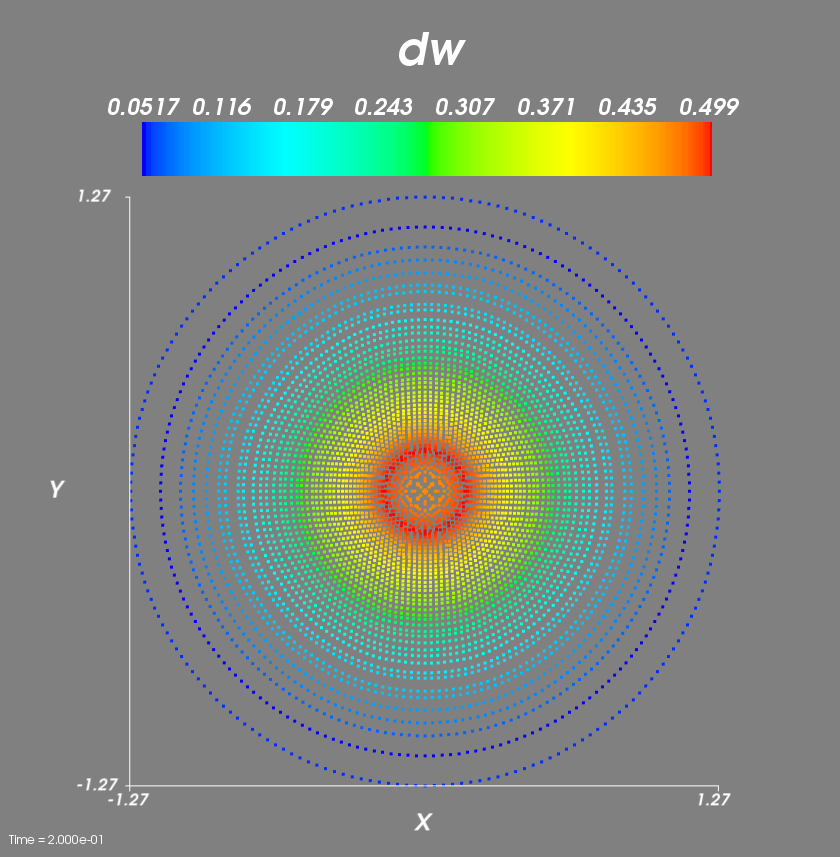
\includegraphics[width=1.1\linewidth]{width_t2.png}
  \caption{t = 0.2 s}
  \label{fig:su3}
\end{subfigure}%
\begin{subfigure}{.5\textwidth}
  \centering
  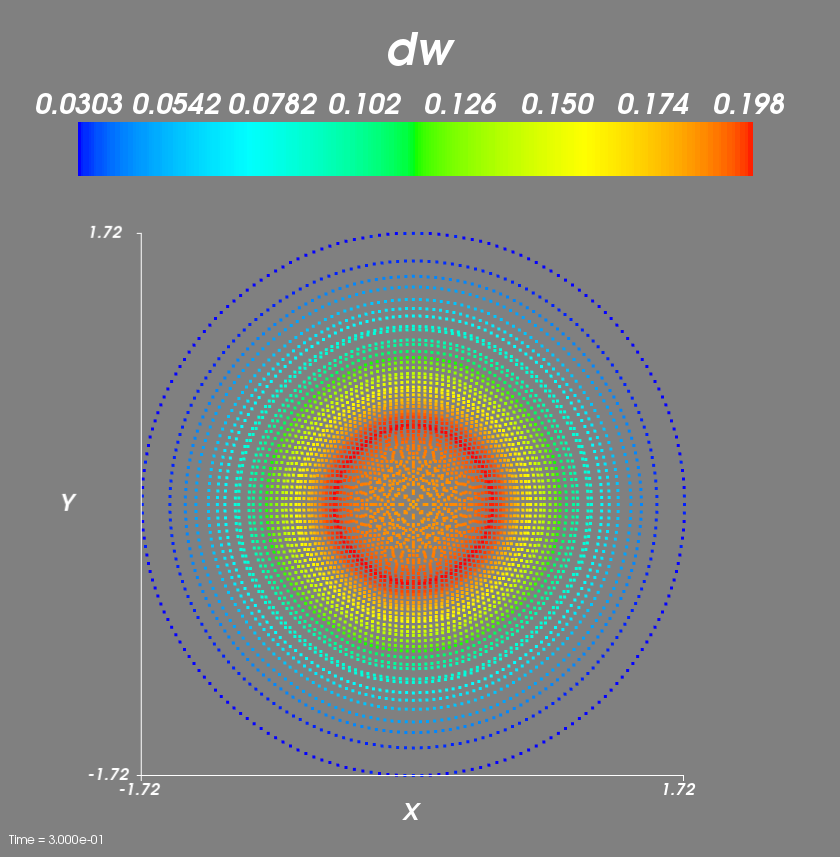
\includegraphics[width=1.1\linewidth]{width_t3.png}
  \caption{t = 0.3 s}
  \label{fig:su4}
\end{subfigure}
\caption{Top View of a Collapsing Water Column (The color represents height of column in m)}
\label{fig:topcollapse}
\end{figure}
\newpage
\subsection{Comparison with dam break collapse using Weakly Compressible Scheme}
\begin{itemize}
\item Due to the presence of viscosity when using the WC scheme, the dam breaks
much slowly than the above simulation result. Once the dissipative friction
term is added to the SWE-SPH model, I will compare it with the WC scheme.
\end{itemize}
\begin{figure}[!htbp]
\centering
\begin{subfigure}{.5\textwidth}
  \centering
  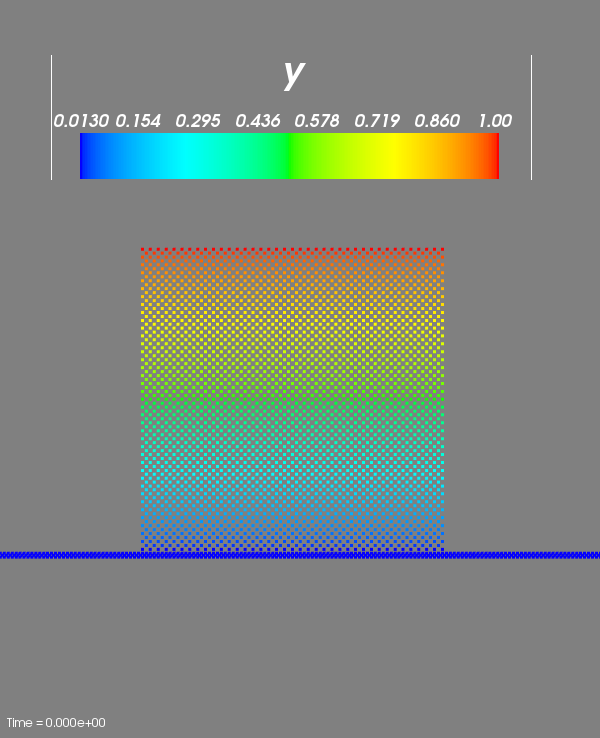
\includegraphics[width=0.8\linewidth]{wc_t0.png}
  \caption{t = 0 s}
  \label{fig:su1}
\end{subfigure}%
\begin{subfigure}{.5\textwidth}
  \centering
  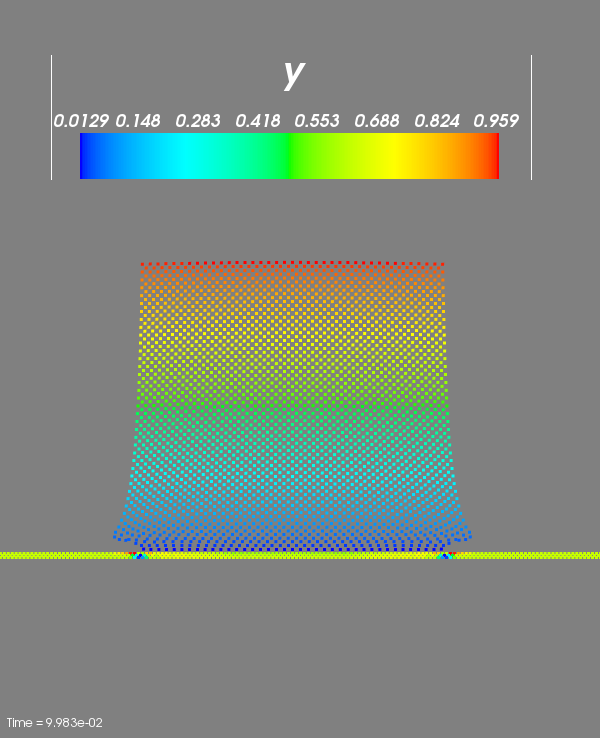
\includegraphics[width=0.8\linewidth]{wc_t1.png}
  \caption{t = 0.1 s}
  \label{fig:su2}
\end{subfigure}
\begin{subfigure}{.5\textwidth}
  \centering
  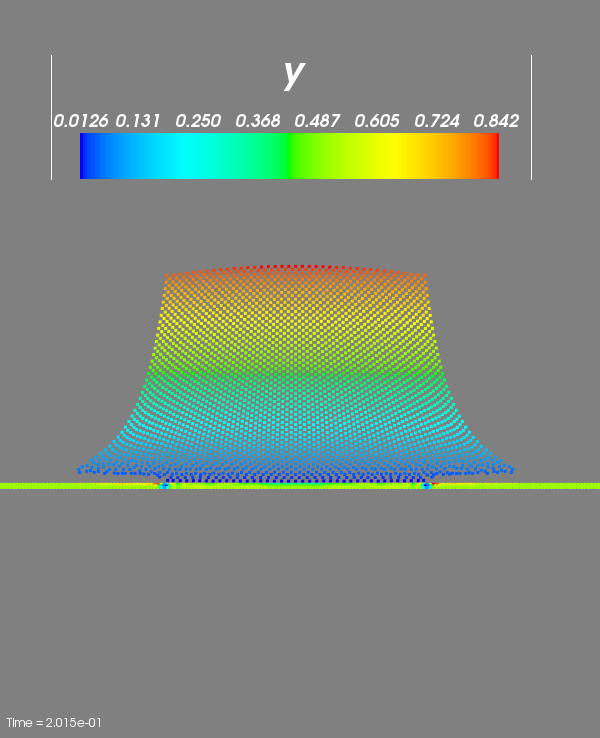
\includegraphics[width=0.8\linewidth]{wc_t2.png}
  \caption{t = 0.2 s}
  \label{fig:su3}
\end{subfigure}%
\begin{subfigure}{.5\textwidth}
  \centering
  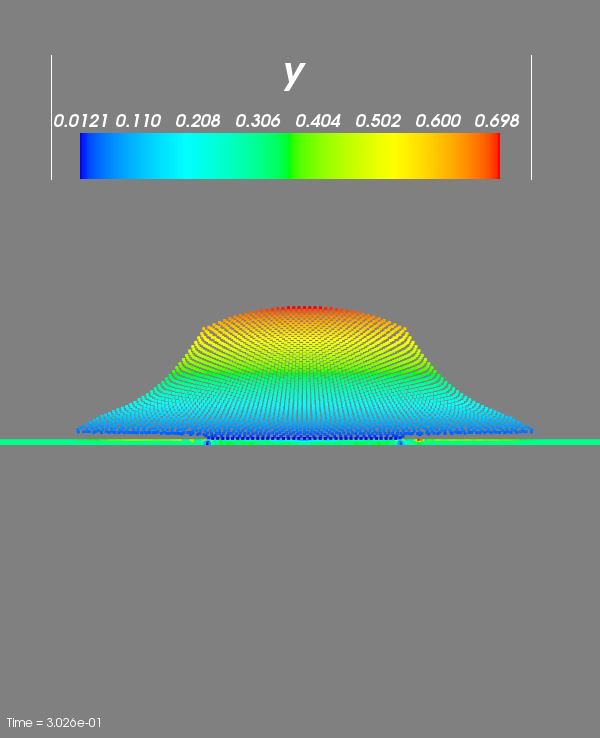
\includegraphics[width=0.8\linewidth]{wc_t3.png}
  \caption{t = 0.3 s}
  \label{fig:su4}
\end{subfigure}
\caption{Side View of a Collapsing Water Column using Weakly Compressible Scheme}
\label{fig:sidecollapsewc}
\end{figure}


\section{Rectangular Dam Break Collapse using Newton-Raphson Variable-h SPH}
A rectangular dam of height 1m, width 1m and length 4m is made to collapse on a 
horizontal surface. The following are the results obtained on comparsion with 
the analytical solution (Ritters Solution).

\subsection{Comparison with Vishnu's Simulation}
\begin{figure}[!htbp]
\centering
\begin{subfigure}{.5\textwidth}
  \centering
  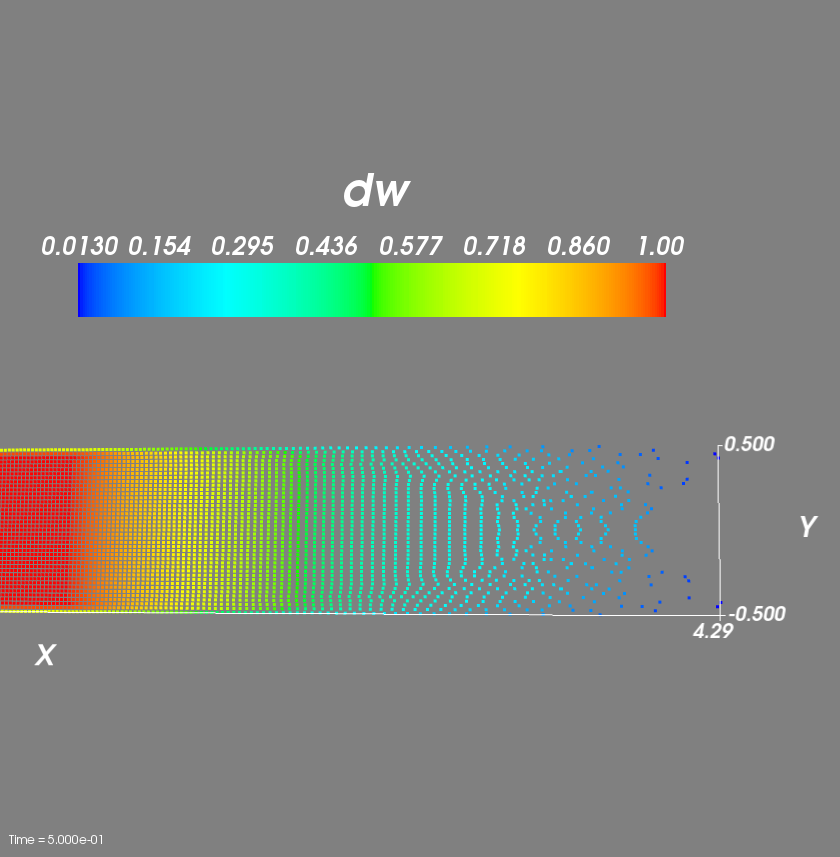
\includegraphics[width=0.8\linewidth]{vishnu_rectdam.png}
  \caption{Vishnu Simulation}
  \label{fig:r11}
\end{subfigure}%
\begin{subfigure}{.5\textwidth}
  \centering
  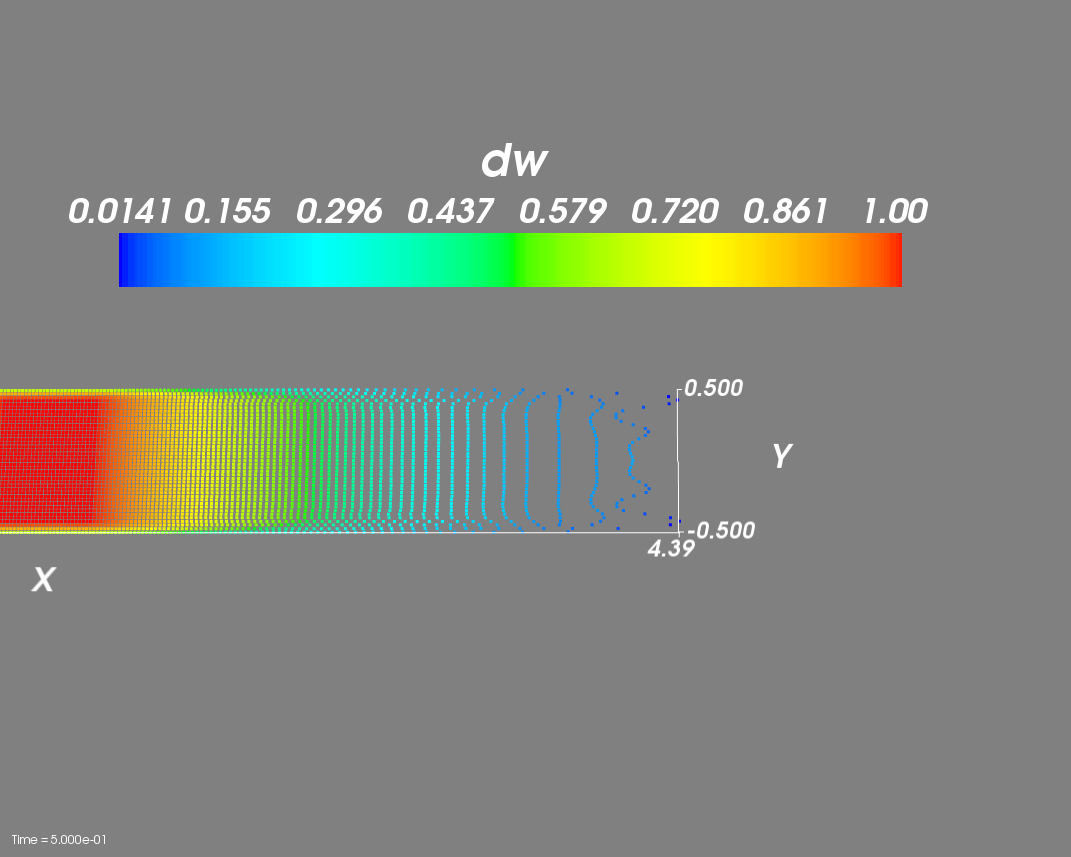
\includegraphics[width=1.0\linewidth]{my_rectdam.png}
  \caption{SWE-SPH Newton-Raphson Iteration}
  \label{fig:r21}
\end{subfigure}
\caption{Collapse of rectangluar dam at t = 0.5s}
\label{fig:rect}
\end{figure}

\newpage
\subsection{Comparison with Analytical Solution}
The velocity and height of the dam at the gate is found to be constant till the 
backward travelling wave reaches the position x = 0.\\
\\
The height of the dam at the gate is given by $\dfrac{4}{9}h_o$\\
The velocity of the dam at the gate is given by $\dfrac{2}{3}\sqrt{gh_o}$

\begin{figure}[!htbp]
\centering
\begin{subfigure}{.5\textwidth}
  \centering
  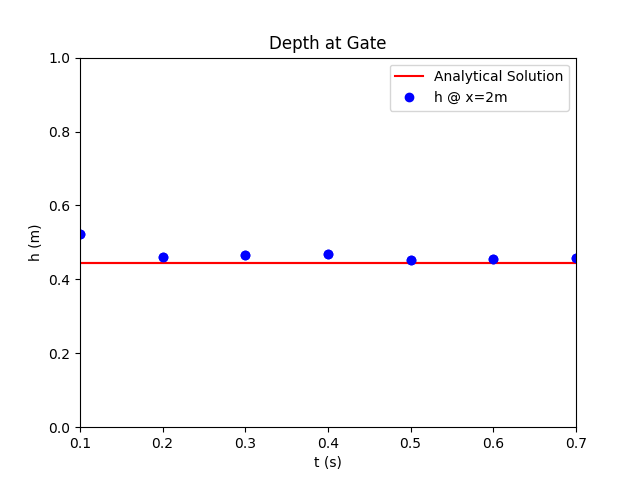
\includegraphics[width=1.1\linewidth]{depth_gate.png}
  \caption{}
  \label{fig:s11}
\end{subfigure}%
\begin{subfigure}{.5\textwidth}
  \centering
  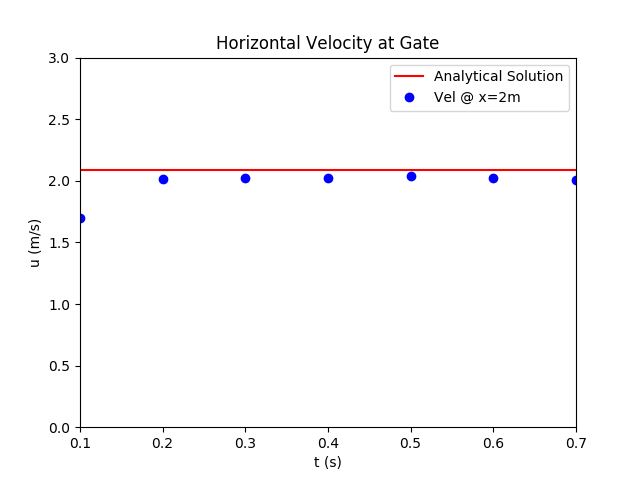
\includegraphics[width=1.1\linewidth]{Vel_gate.png}
  \caption{}
  \label{fig:s21}
\end{subfigure}
\begin{subfigure}{.5\textwidth}
  \centering
  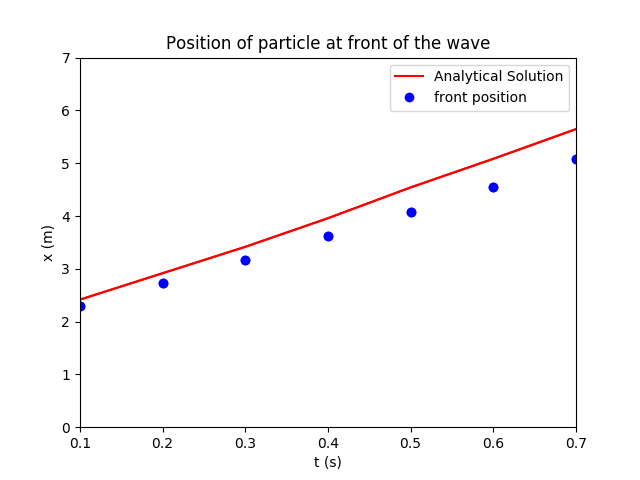
\includegraphics[width=1.1\linewidth]{wavefront_position_anal_is_from_rodri.png}
  \caption{}
  \label{fig:s31}
\end{subfigure}
\caption{Comparsion of depth and velocity at the gate with Analytical Solution}
\label{fig:rect1}
\end{figure}

\newpage
The analytical expression for the profile of the dam is given by 
\begin{equation}
    x = t[2\sqrt(gh_o) - 3\sqrt(gh)]
    \label{}
\end{equation}
where,
\begin{align*}
    x &- \text{Distance measured from the dam gate}\\
    h &- \text{Height of the dam after time t}\\
    h_0 &- \text{Initial height of dam}\\
    g &- \text{Acceleration due to gravity}\\
\end{align*}
\begin{figure}[!htbp]
\centering
\begin{subfigure}{.5\textwidth}
  \centering
  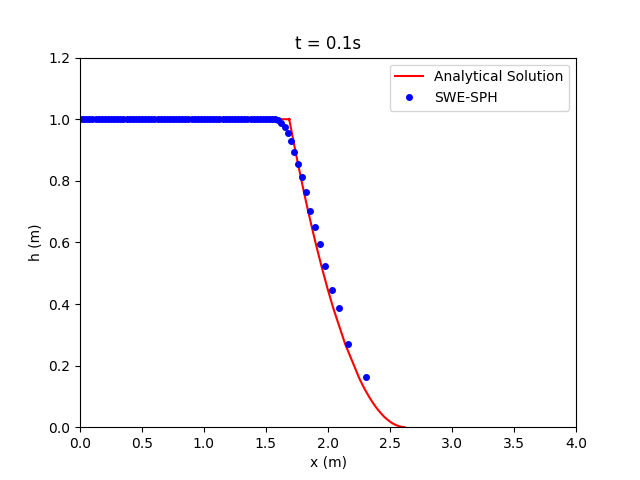
\includegraphics[width=1.1\linewidth]{depth_pos_01.png}
  \caption{t = 0.1 s}
  \label{fig:sun1}
\end{subfigure}%
\begin{subfigure}{.5\textwidth}
  \centering
  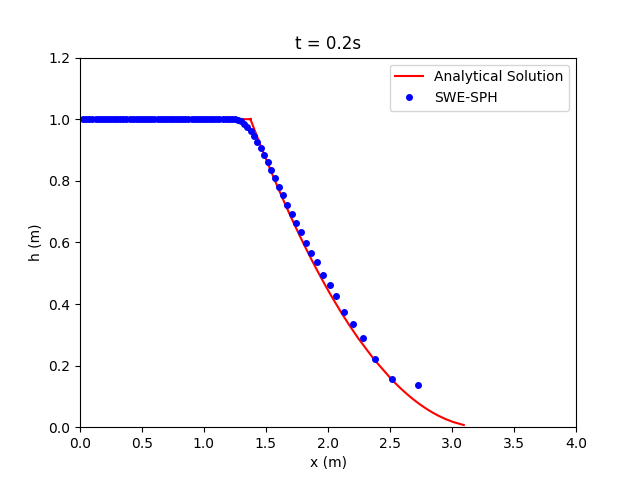
\includegraphics[width=1.1\linewidth]{depth_pos_02.png}
  \caption{t = 0.2 s}
  \label{fig:sun2}
\end{subfigure}
\begin{subfigure}{.5\textwidth}
  \centering
  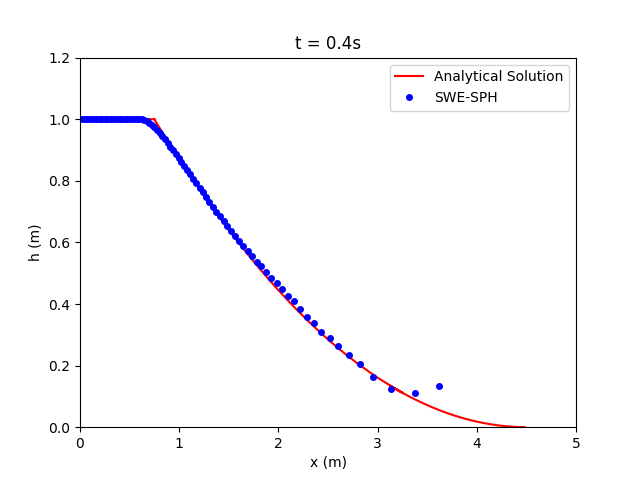
\includegraphics[width=1.1\linewidth]{depth_pos_04.png}
  \caption{t = 0.4 s}
  \label{fig:sun3}
\end{subfigure}%
\begin{subfigure}{.5\textwidth}
  \centering
  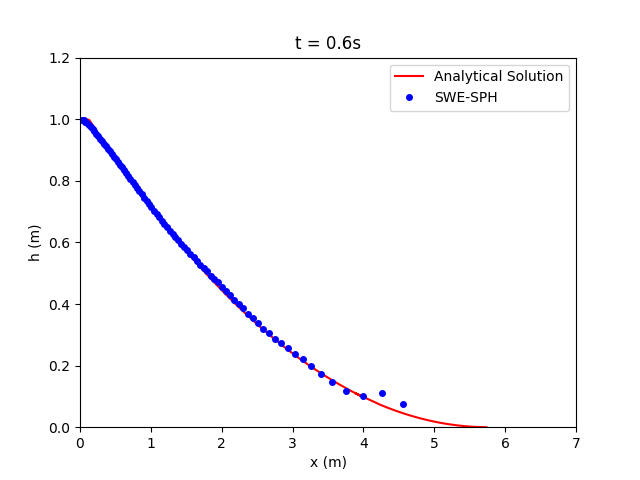
\includegraphics[width=1.1\linewidth]{depth_pos_06.png}
  \caption{t = 0.6 s}
  \label{fig:sun4}
\end{subfigure}
\caption{Dam break profile at various times}
\label{fig:rect2}
\end{figure}




\end{document}
